\documentclass[a4paper]{article}
\usepackage{amsmath}
\DeclareMathOperator*{\argmax}{arg\,max}
\DeclareMathOperator*{\argmin}{arg\,min}
\usepackage{amssymb}
\usepackage{amsthm}
\usepackage{graphicx}
\usepackage{float}
\newtheorem{theorem}{Theorem}[section]
\newtheorem{lemma}{Lemma}[section]

\title{Beta Distribution}
\author{listenzcc}

\begin{document}

\maketitle

\abstract
Bayesian learning is an active field of machine learning.
It estimates parameters of known distribution rather than calculates coefficients directly.
This article is a shallow instance of Bayesian learning.
It shows how to estimate success rate with strong prior knowledge in Bernoulli experiment.
Inevitably, it involves Beta distribution, Bernoulli distribution and their relationship of being conjugate prior pair.
Additionally, it contains the calculation of the integral of Beta function using $\Gamma$ function, which provides an easy path to calculate the expectation of mean and variance of Beta distribution.

\tableofcontents

\section{Beta distribution}
The \emph{Beta distribution} can be used to a conjugate prior\footnote{Conjugate prior. Suppose we have data with likelihood function $f(x|\theta)$ depending on a hypothesized parameter. Also suppose the prior distribution for $\theta$ is one of a family of parametrized distributions. If the posterior distribution for $\theta$ is in this family then we say the the prior is a conjugate prior for the likelihood.} to \emph{Bernoulli distribution}.

\subsection{Definition}
The probability function $P(x)$ of Beta distribution is defined as proportional to the function of $x \in (-\infty, \infty)$
\begin{equation}
    P(x) \propto x^{\alpha-1} (1-x)^{\beta-1}
\end{equation}
there are two prior parameters, $\alpha$ and $\beta$ controlling the shape of the distribution.

To guarantee that the integral of $P(x)$ is $1$, and we have
\begin{equation}
    P(x) = \frac{x^{\alpha-1} (1-x)^{\beta-1}}{B(\alpha, \beta)}
\end{equation}
where $B(\alpha, \beta)$ is Beta function.
The guarantee is based on a theorem, we will prove it in later.

Thus, the probability density function of Beta distribution can be expressed as 
\begin{equation}
    Beta(x; \alpha, \beta) = \frac{x^{\alpha-1} (1-x)^{\beta-1}}{B(\alpha, \beta)}
\end{equation}

The overlook of Beta distribution among different parameters combinations is drawn as Fig.\ref{fig: Beta distribution}.
\begin{figure}[H]
    \centering
    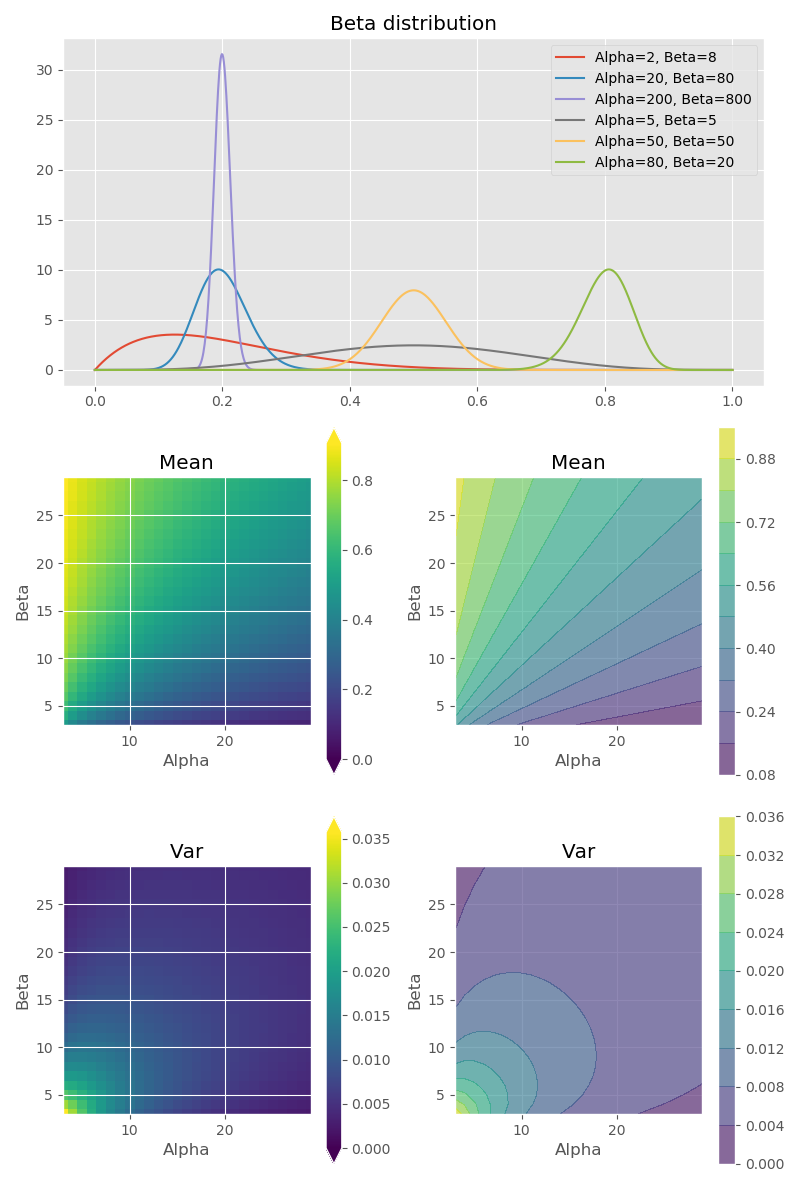
\includegraphics[height=0.5\textheight]{beta_distribution.png}
    \caption{Beta distribution among different parameters combinations}
    \label{fig: Beta distribution}
\end{figure}

\section{Beta function}
The \emph{Beta function}\footnote{Beta function is also known as Euler's integral of the first kind} is important in calculus and analysis due to its close connection to the $\Gamma$ function, which is itself a generalization of the factorial function.
Many complex integrals can be reduced to expressions involving the beta function.

\subsection{Definition}
The Beta function, denoted by $B(x, y)$, is defined as
\begin{equation}
    B(\alpha, \beta) := \int_{0}^{1} t^{\alpha-1} (1-t)^{\beta-1} dt
    \label{eq: Beta function}
\end{equation}
it is definite integrals.

\subsection{Theorem}

\begin{theorem}
    Beta function is symmetry
    \begin{equation}
        B(\alpha, \beta) = B(\beta, \alpha)
    \end{equation}

    \begin{proof}
        Because of the convergent property of definite integrals
        \begin{equation*}
            \int_{0}^{a} f(t) dt = \int_{0}^{a} f(a-t) dt
        \end{equation*}
        so we can rewrite the integral (\ref{eq: Beta function}) as
        \begin{equation*}
            B(\alpha, \beta) = \int_{0}^{1} t^{\beta-1} (1-t)^{\alpha-1} dt
        \end{equation*}

        Thus, we get that Beta function is symmetric, $B(\alpha, \beta) = B(\beta, \alpha)$.
    \end{proof}

\end{theorem}

\begin{theorem}
    The integral of Beta function can be calculated using $\Gamma$ function.
    \begin{equation}
        B(\alpha, \beta) = \frac{\Gamma(\alpha)\Gamma(\beta)}{\Gamma(\alpha+\beta)}
    \end{equation}
    where $\Gamma$ function is defined as
    \begin{equation}
        \Gamma(\alpha) = \int_{0}^{\infty} t^{\alpha-1} e^{-t} dt
        \label{eq: Gamma function}
    \end{equation}

    \begin{proof}
        One can write
        \begin{equation*}
            \Gamma(m)\Gamma(n) = \int_{0}^{\infty} x^{m-1} e^{-x} dx \int_{0}^{\infty} y^{n-1} e^{-y} dy
        \end{equation*}
        Then rewrite it as a double integral
        \begin{equation*}
            \Gamma(m)\Gamma(n) = \int_{0}^{\infty} \int_{0}^{\infty} x^{m-1} y^{n-1} e^{-x-y} dx dy
        \end{equation*}
        Applying the substitution $x=vt$ and $y=v(1-t)$, we have
        \begin{equation*}
            \Gamma(m)\Gamma(n) = \int_{0}^{1} t^{m-1} (1-t)^{n-1} dt \int_{0}^{\infty} v^{m+n-1} e^{-v} dv
        \end{equation*}
        Using the definitions of $\Gamma$ and Beta functions, we have
        \begin{equation*}
            \Gamma(m)\Gamma(n) = B(m, n) \Gamma(m+n)
        \end{equation*}
        Hence proved.
    \end{proof}
\end{theorem}

\begin{lemma}
    For positive integer $\alpha$ and $\beta$, Beta function can be expressed as
    \begin{equation}
        B(\alpha, \beta) = \frac{(\alpha-1)!(\beta-1)!}{(\alpha+\beta-1)!}
    \end{equation}
    since $\Gamma(\alpha) = (\alpha-1)!$ when $\alpha \in [1, 2, \ldots]$
\end{lemma}

\section{Bernoulli distribution}

\subsection{Definition}
The \emph{Bernoulli distribution} is a discrete distribution having two possible outcomes labelled by $y=(0, 1)$ in which $y=0$ ("success") occurs with probability $p$ and $n=0$ ("failure") occurs with probability $q=1-p$, where $0 \leq p \leq 1$. It therefore has probability density function.

In an experiment, the probability of obtaining output of $Y$ is
\begin{equation}
    P(y) = p^y (1-p)^{1-y}
\end{equation}

In $N$ experiments, the probability of obtaining $n$ successes is
\begin{equation}
    P(N, n) = \binom{N}{n} p^n (1-p)^{N-n}
\end{equation}

To estimate the value of $p$ based on $N$ and $n$, we can apply MLE \footnote{MLE: Maximum Likelihood Estimation} method, in this case MLE is to solve $p = \hat{p}$ when it maximizes $P(N, n)$.
\begin{equation}
    \hat{p} = \argmax_{p} P(N, n)
\end{equation}

The solution can be obtained with $\frac{\partial}{\partial{\hat{p}}} P(N, n) = 0$ yields $\hat{p} = \frac{n}{N}$.
We will explain why in the following.

\section{Beta and Bernoulli distributions}

\subsection{Bayes' Theorem and Conditional Probability}
\emph{Bayes' theorem} is a formula that describes how to update the probabilities of hypotheses when given evidence. It follows simply from the axioms of conditional probability, but can be used to powerfully reason about a wide range of problems involving belief updates.

Given a hypothesis $H$ and evidence $E$, Bayes' theorem states that the relationship between the probability of the hypothesis before getting the evidence $P(H)$ and the probability of the hypothesis after getting the evidence $P(H|E)$ is
\begin{equation}
    P(H|E) = \frac{P(E|H) P(H)}{P(E)}
\end{equation}
where $P(H|E)$ is the posterior probability, conditional probability of the hypothesis given the evidence, and $P(E|H)$ is the posterior probability of the evidence being obtained when applying the hypothesis.
The $P(E)$ is the universal probability of the evidence, which is usually difficult to know the exact value.

Many modern \emph{machine learning} techniques rely on Bayes' theorem. For instance, spam filters use Bayesian updating to determine whether an email is real or spam, given the words in the email. Additionally, many specific techniques in statistics, such as calculating \emph{p-values} or \emph{interpreting medical results}, are best described in terms of how they contribute to updating hypotheses using Bayes' theorem.

\subsection{Conjugate prior}

In a Bernoulli experiment, if we repeat the experiment $N$ times, and obtain $n$ successes.
The estimation of $p$ value is usually the first important problem to solve.
Traditional method can give an estimation as $\hat{p}=\frac{n}{N}$, however it seems too arbitrary when $N$ is small, and has ignored the useful of prior probability.

Here we try to estimate the value of $p$ using Bayes' theorem.
Firstly, we have an assumption that $p$ fits Beta distribution with parameters of $\alpha$ and $\beta$
\begin{equation}
    Beta(p; \alpha, \beta) = \frac{p^{\alpha-1} (1-p)^{\beta-1}}{B(\alpha, \beta)}
\end{equation}

The expectation of mean and variance of $p$ is obvious when $\alpha$ and $\beta$ are positive integers.
\begin{equation}
    E(p) = \frac{\alpha}{\alpha+\beta}
\end{equation}
\begin{equation}
    D(p) = \frac{\alpha\beta}{(\alpha+\beta+1)(\alpha+\beta)^2}
    \label{eq: variance of Beta function}
\end{equation}


\begin{proof}
    Start from the definition of expectation
    \begin{equation*}
        E(P) = \int_{0}^{1} p Beta(p; \alpha, \beta) dp
    \end{equation*}
    it is easy to calculate the integral of the numerator is $B(\alpha+1, \beta)$.
    Thus the exception can be calculated by
    \begin{equation*}
        E(P) = \frac{B(\alpha+1, \beta)}{B(\alpha+\beta)} = \frac{\alpha}{\alpha+\beta}
    \end{equation*}

    One can obtain the variance following
    \begin{equation*}
        D(P) = E(P^{2}) - E^{2}(P)
    \end{equation*}
    where $E^{2}(P)$ is obvious and $E(P^{2})$ can be calculated as
    \begin{equation*}
        E(P^{2}) = \int_{0}^{1} p^{2} Beta(p; \alpha, \beta) dp = \frac{B(\alpha+2, \beta)}{B(\alpha+\beta)} = \frac{(\alpha+1)\alpha}{(\alpha+\beta+1)(\alpha+\beta)}
    \end{equation*}
    thus, we have
    \begin{equation*}
        D(p) = \frac{(\alpha+1)\alpha}{(\alpha+\beta+1)(\alpha+\beta)} - \frac{\alpha\alpha}{(\alpha+\beta)(\alpha+\beta)}
    \end{equation*}

\end{proof}

Suppose we have a prior assumption that probability of success is $p$.
The posterior probability of the $n$ successes outcome is
\begin{equation}
    P(E|H) = \binom{N}{n} p^n (1-p)^{N-n}
\end{equation}
where $H$ refers the assumption that probability of success is $p$, $E$ refers obtaining $n$ successes out of $N$ experiments.

We can write prior probability as following
\begin{equation}
    P(H) \propto p^{\alpha-1} (1-p)^{\beta-1}
    \label{eq: Prior probability}
\end{equation}

Applying Bayes' theorem we have
\begin{equation}
    P(H|E) = \frac{P(E|H) P(H)}{P(E)} = p^n (1-p)^{N-n} \cdot p^{\alpha-1} (1-p)^{\beta-1} \mathcal \cdot \mathcal{C}
\end{equation}
where the denominator is simplified as a constant $\mathcal{C}$. The simplify is reasonable since the $P(E)$ is invariant with respect to $p$, despite its difficulty to solve.

It turns out that $P(H|E)$ is proportional to Beta function family as following
\begin{equation}
    P(H|E) \propto p^{n + \alpha - 1} (1-p)^{N - n + \beta - 1}
\end{equation}
applying substitution of $\alpha^{'} = n + \alpha$ and $\beta^{'} = N - n + \beta$, and denominator of Beta function, we have
\begin{equation}
    P(H|E) = \frac{p^{\alpha^{'}-1} (1-p)^{\beta^{'}-1}}{B(\alpha^{'}, \beta^{'})}
    \label{eq: Posterior probability}
\end{equation}
we can see that the posterior probability $P(H|E)$ and prior probability $P(H)$ are from the same distribution family.

\subsection{Bayesian learning}
The way we apply Bayes' theorem using conjugate prior is the idea of Bayesian learning.
We can not say which is better, Bayesian learning or MLE.
However, we can say the Bayesian learning method is more stable since it yields smaller variance.
The smaller variance is because Bayesian learning method uses the prior knowledge (\ref{eq: Prior probability}).
In prior, we assumed that $p$ is variable and centered on the point of $\frac{\alpha}{\alpha + \beta}$.
After we obtained the evidence that $n$ out of $N$ successes, we formulate a closer estimation in (\ref{eq: Posterior probability}).
It can be found that the new estimation has much lower variance (\ref{eq: variance of Beta function}), since $\alpha^{'} > n$ and $\alpha^{'} + \beta^{'} > N$.

This explains another different between MLE and Bayesian learning method.
MLE is more like a pure data driven method, it estimate coefficients based on only observed data.
Bayesian learning uses data as adjustment for prior, the more data obtained the larger adjustment can be made.
The adjustment strategy may provide a robust estimation against arbitrary noisy.

\end{document}